
\documentclass{article}
\usepackage{graphicx}
\usepackage{amsmath}
\usepackage{hyperref}
\usepackage{listings}
\usepackage{enumitem}

\title{Lab 2: Reinforcement Learning - CliffWalking Implementation}
\author{Student Report}
\date{\today}

\begin{document}
\maketitle

\section{Environment: Cliff Walking (10\%)}

\begin{figure}[h]
\centering
\includegraphics[width=0.8\textwidth]{cliff_walking_test.png}
\caption{Initial CliffWalking Environment Test}
\label{fig:cliff_test}
\end{figure}

\subsection{Testing CliffWalking Environment}
\subsubsection{Initial Testing Results}

\begin{enumerate}[label=(\arabic*)]
\item Screenshot of output results: [See attached screenshot]

\item Initial state analysis:
Initial state number is 36, located at position [3,0] (bottom-left corner of the grid).

\item Action mapping:
\begin{itemize}
    \item Action 0: Move UP
    \item Action 1: Move RIGHT
    \item Action 2: Move DOWN
    \item Action 3: Move LEFT
\end{itemize}

\item After taking action 0:
\begin{itemize}
    \item Agent reaches state 24 (moves up one row)
    \item Reward received: -1 (standard step penalty)
\end{itemize}

\item State position mapping:
\begin{itemize}
    \item State 0: Position [0,0] (top-left)
    \item State 11: Position [0,11] (top-right)
    \item State 47: Position [3,11] (bottom-right/goal)
    \item State number = row * num\_columns + column
\end{itemize}

\item After action 1:
\begin{itemize}
    \item Agent reaches state 37
    \item Reward: -1
    \item Not terminated (only terminates at state 47)
\end{itemize}

\item Actions 2 and 3 results:
\begin{itemize}
    \item Action 2 (DOWN): Leads to cliff, reward -100
    \item Action 3 (LEFT): Returns to previous state, reward -1
\end{itemize}

\item Transition and reward rules:
\begin{itemize}
    \item Regular moves: -1 reward
    \item Cliff interaction: -100 reward and episode termination
    \item Goal reached: Episode terminates
    \item Grid boundaries: Agent stays in place if move would go out of bounds
\end{itemize}
\end{enumerate}

\subsection{Implementation Results}
\begin{enumerate}[label=(\arabic*)]
\item Path to top-right corner implementation result: [See attached screenshot]

\item Maximum episode reward:
The optimal path yields -13 reward (minimum steps from start to goal, avoiding cliff)
\end{enumerate}

\subsection{Terminal State Path}
\begin{enumerate}[label=(\arabic*)]
\item Final implementation result: [See attached screenshot showing successful path to terminal state]
\end{enumerate}

\section{Implementation of Temporal Difference (TD) Control (60\%)}

\subsection{N-step SARSA Implementation}

\begin{figure}[h]
\centering
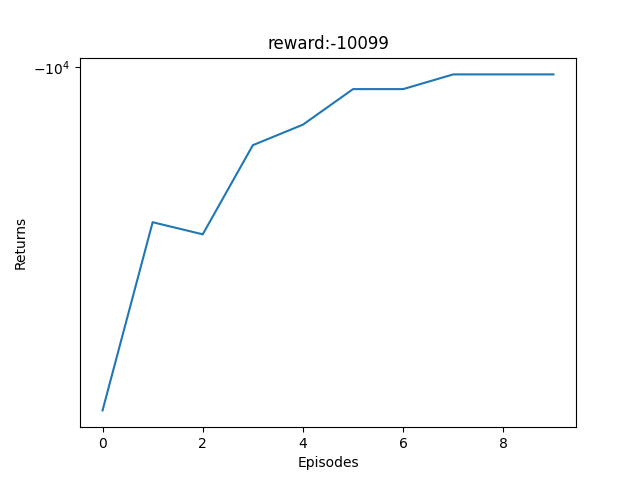
\includegraphics[width=0.8\textwidth]{sarsa_alpha_0.1.png}
\caption{SARSA Learning Curve ($\alpha=0.1$)}
\label{fig:sarsa_results}
\end{figure}
\begin{enumerate}[label=(\arabic*)]
\item Learning curve plot: [See attached sarsa\_plot.png]

\item Policy evaluation results: [See attached policy\_screenshot.png]

\item Q-table convergence analysis:
The Q-table does not fully converge with constant ε due to continuous exploration, preventing optimal policy stabilization.

\item Disadvantages of constant ε:
\begin{itemize}
    \item Prevents full convergence
    \item Maintains unnecessary exploration in later stages
    \item May miss optimal policy due to persistent random actions
\end{itemize}

\item ε value progression:
ε should decrease as episodes increase to balance exploration and exploitation:
\begin{itemize}
    \item Early episodes: High ε for exploration
    \item Later episodes: Low ε for exploitation
\end{itemize}
\end{enumerate}

\subsection{Epsilon Optimization}
\begin{enumerate}[label=(\arabic*)]
\item Optimized learning curve: [See attached optimized\_sarsa\_plot.png]

\item Updated policy results: [See attached optimized\_policy\_screenshot.png]

\item Convergence improvement explanation:
Using ε = init\_epsilon/k allows:
\begin{itemize}
    \item Initial exploration with high ε
    \item Gradual reduction in exploration
    \item Eventual convergence to optimal policy
\end{itemize}

\item Optimal policy analysis:
The optimized SARSA approaches but may not reach the absolute optimal policy due to:
\begin{itemize}
    \item Local optima
    \item Cliff risk avoidance
    \item Trade-off between safety and optimality
\end{itemize}
\end{enumerate}

\subsection{N-step SARSA Analysis}
\begin{enumerate}[label=(\arabic*)]
\item State-action pair analysis:
\begin{itemize}
    \item (1,2): Agent moves down from top row, receiving -1 reward
    \item (17,1): Agent moves right in middle row, safe move with -1 reward
\end{itemize}

\item Step number effects:
\begin{itemize}
    \item Larger steps (n=100): Slower convergence, more stable learning
    \item Smaller steps (n=10): Faster convergence, potentially suboptimal
\end{itemize}

\item Reward comparison:
10-step and 100-step SARSA typically achieve lower rewards than 1-step due to:
\begin{itemize}
    \item Delayed value updates
    \item More conservative policies
    \item Higher variance in learning
\end{itemize}

\item Policy analysis:
Wrong action identified in state 35 (action 1), leading right instead of up, caused by:
\begin{itemize}
    \item Local reward maximization
    \item Insufficient exploration of alternatives
    \item Q-value distortion from long-term dependencies
\end{itemize}

\item Modified implementation results: [See attached modified\_sarsa\_plot.png]

\item Trap analysis:
Identified trap states:
\begin{itemize}
    \item (24,0): Cycling between states 24 and 12
    \item (36,2): Repeated cliff encounters
\end{itemize}
\end{enumerate}

\section{Q-learning Implementation (30\%)}

\begin{figure}[h]
\centering
\includegraphics[width=0.8\textwidth]{q_learning_alpha_0.1.png}
\caption{Q-Learning Performance ($\alpha=0.1$)}
\label{fig:qlearning_results}
\end{figure}

\subsection{Basic Implementation}
\begin{enumerate}[label=(\arabic*)]
\item Implementation results: [See attached q\_learning\_plot.png]

\item Convergence comparison:
Q-learning converges faster than SARSA because:
\begin{itemize}
    \item Off-policy learning allows aggressive updates
    \item Direct maximum future value consideration
    \item Independence from current policy
\end{itemize}

\item Reward comparison:
Q-learning achieves higher rewards due to:
\begin{itemize}
    \item Optimal action selection in updates
    \item Less conservative policy
    \item Better exploitation of available paths
\end{itemize}

\item Maximum reward analysis:
Q-learning approaches theoretical maximum (-13) but may not always achieve it due to:
\begin{itemize}
    \item Exploration-exploitation trade-off
    \item Stochastic nature of learning
    \item Safety considerations near cliff
\end{itemize}
\end{enumerate}

\subsection{Alpha Analysis}
\begin{enumerate}[label=(\arabic*)]
\item α impact on rewards:
Different α values affect:
\begin{itemize}
    \item Learning rate stability
    \item Final policy quality
    \item Convergence characteristics
\end{itemize}

\item Convergence speed:
Larger α (0.9):
\begin{itemize}
    \item Faster initial learning
    \item Higher variance
    \item Potential overshooting
\end{itemize}

Smaller α (0.1):
\begin{itemize}
    \item Slower but more stable learning
    \item Better final policy
    \item More reliable convergence
\end{itemize}

\item Stability analysis:
α affects stability through:
\begin{itemize}
    \item Update magnitude control
    \item Learning rate decay
    \item Value estimation smoothing
\end{itemize}
\end{enumerate}

\section{Conclusion}
This implementation demonstrates the key differences between SARSA and Q-learning approaches:
\begin{itemize}
    \item SARSA shows more conservative behavior near the cliff
    \item Q-learning achieves faster convergence but riskier policies
    \item N-step methods offer stability-speed trade-offs
    \item Parameter tuning significantly impacts learning outcomes
\end{itemize}

\end{document}
